\chapter{Background subtraction}
\section{Assessing Beamline Contamination}
What is the beamline contamination? We define beamline contamination every TPC track matched to the WC track which is not a primary pion. There are 4 different types of beamline contaminations:
\begin{itemize}
\item[]1) electrons,
\item[]2) muons,
\item[]3) secondaries from pion events,
\item[]4) matched pile up events.
\end{itemize}

So, how do we handle this contamination?
The first step is to estimate what percentage of events used in the cross section calculation is not a primary pion.  

\subsection{Electron and Muon contamination}
We estimate the percentage of electrons and muons in the beam via the beamline MC. 
Since the beamline composition is a function of the magnet settings, we simulate separately events for magnet current of -60A and -100A. 

\begin{figure}
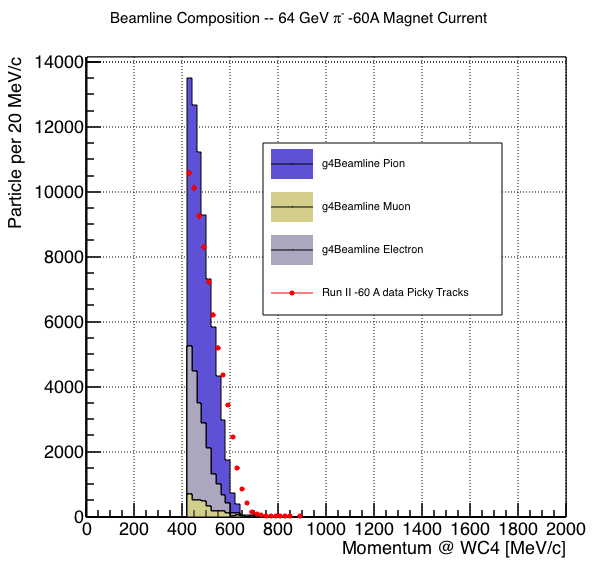
\includegraphics[width=0.5\textwidth,height=\textheight,keepaspectratio]{Chapter-7/Images/Beam60A.png}
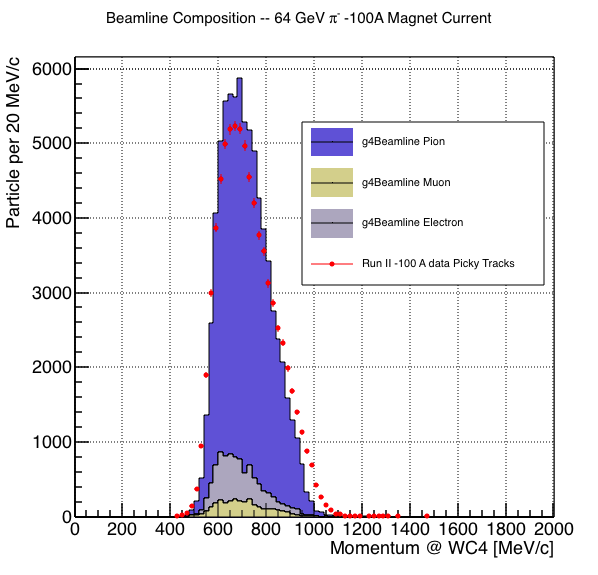
\includegraphics[width=0.5\textwidth,height=\textheight,keepaspectratio]{Chapter-7/Images/Beam100A.png}
\label{fig:BeamComposition}
\caption{Beam composition for the -60A runs (left) and -100A runs (right). The solid blue plot represents the pion content, the yellow plot represents the muon content and the grey plot represents the electron content. The plots are area normalized to the number of data events, shown in red. }
\end{figure}

Table \ref{tab:beamline} shows the beam composition per magnet setting after the mass selection according to the G4simulation, 
\begin{table}[]
\centering
\label{tab:beamline}
\begin{tabular}{|l|c|c|}
\hline
                     & I = -60 A           & I = -100 A \\ \hline
G4Pions       &   68.8 \%           &      87.4 \%        \\ \hline
G4Muons     &     4.6 \%           &        3.7 \%         \\ \hline
G4Electrons &   26.6 \%           &        8.9 \%        \\ \hline
\end{tabular}
\caption{Beamline composition per magnet settings}
\end{table}


\begin{table}[]
\centering
\label{tab:databreakdown}
\begin{tabular}{|l|c|c|c|c|c|}
\hline
                                                     & I = -60 A          & I = -100 A   & Total     &  w$_{60A}$ &  w$_{100A}$\\ \hline
Data events after Mass Cut         &     70192          &  76056       & 146248 & 0.52 & 0.48\\ \hline
Data events for Cross Section     &                         &                   &              & & \\ \hline
\end{tabular}
\caption{Data events per magnet settings}
\end{table}



We calculate the electron to pion and muon to pion ratio on the whole sample as the weighted sum of the corresponding ratio in the two current settings, 
\begin{equation}
\frac{N_e}{N_\pi}_{Data} = w_{60A}\frac{N_e}{N_\pi}_{60A}  + w_{100A}\frac{N_e}{N_\pi}_{100A},
\end{equation}
\begin{equation}
\frac{N_\mu}{N_\pi}_{Data} = w_{60A}\frac{N_\mu}{N_\pi}_{60A}  + w_{100A}\frac{N_\mu}{N_\pi}_{100A},
\end{equation}
where the weights $w_{60A}$ and $w_{100A}$ are the percentage of events in the corresponding magnet configuration passing the mass selection in data, as shown in \ref{tab:databreakdown}.


Once the beam composition is know,  we simulate the electrons, muons and pions with the DDMC and we subject the three samples to the same selection chain (WC2TPC match, shower filter, pile up filter, etc...). The percentage of electrons and muons surviving the selection chain is the  electron and muon contamination in the pion cross section sample.

\subsection{Contamination from secondaries}
The percentage of secondaries is given in the MC by the number of matched WC2TPC tracks which are not flagged as primary by Geant4.
We estimate the last type of contamination, the ``matched pile up" events, to be a negligible fraction, because of the definition of the WC2TPC match: we deem the probability of a single match with a halo particle in the absence of a beamline particle\footnote{ Events with multiple WC2TPC matches are always rejected.} extremely small.

\section{Subtraction}
Once we estimate the contaminants to primary pion ratio, the next step is subtracting their contribution from data for each type of contaminant independently. The contaminant samples are reconstructed and the corresponding interacting and incident histograms are produced. We then perform a bin by bin subtraction in the data interacting and incident histograms separately. A graphical rendering of this procedure is shown in Fig \ref{fig:backgroundSubtraction}
Once the data is background subtracted, we apply the correction laid out in the previous section.
\textcolor{blue}{How do we account for the error in the contamination subtraction? We change the electron/pion and muon/pion ratio and we see how much difference we get?}

\begin{figure}
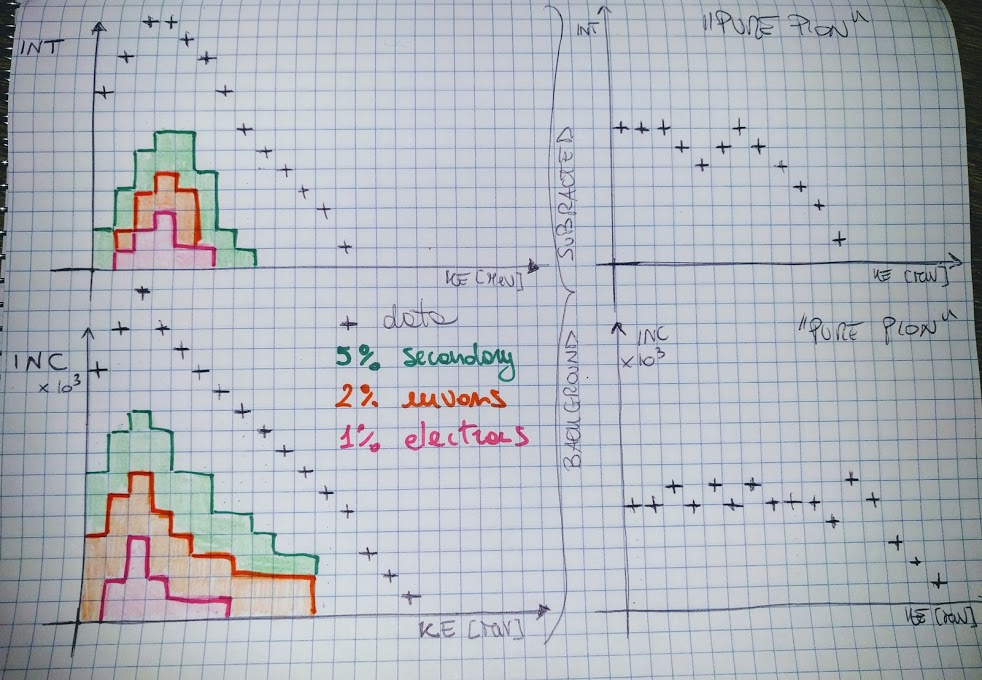
\includegraphics[width=\textwidth,height=\textheight,keepaspectratio]{Chapter-9/Images/FakePlot.jpg}
\label{fig:backgroundSubtraction}
\caption{A graphical rendering of the beamline contamination background subtraction. The contribution of the contaminants is shown in green for the secondaries, in orange for the muons and in pink for electrons. The colored plots are coming from the MC and are staggered. The percentages shown in the legend are the percentages of contaminants over the total number of events  passing the selection chain. We actually expect way less contamination.}
\end{figure}

\section{Capture and decay}\label{ch:CaptureAndDecay}
Our goal is to measure the total hadronic cross section for negative pions in argon. Since pion capture can be classified as an electromagnetic process and pion decay is a week process,  capture and decay represent unwanted interactions. We present here a study of capture and decay in Monte Carlo and the solution we adopted to mitigate their present in the data sample. 

For this MC study, we use a sample of 359000 MC pions generated according to the beam profile with the DDMC described in \ref{sec:DDMC}. It is important to notice that capture occurs predominantly at rest, while decay may occur both in flight and at rest. Thus, we can highly mitigate capture and decay at rest by removing pions which would release all their energy in the TPC and stop. This translates into a momentum selection, where we keep only events whose WC momentum is above a certain threshold. 
Figure \ref{fig:CaptureMom} shows the true momentum distribution for the primary\footnote{We use here the Geant4 denomination ``primary" to indicate that the pion considered does not undergo interactions modifying its energy before getting to the TPC. In fact, not every pion shot from wire chamber four will arrive to the TPC as primary,  some will decay or interact before the TPC.} pions that arrive to the TPC (pink), that capture (green) or decay (blue) inside the TPC, on a linear and log scale vertical axis. 

\begin{figure}[hpbt]
\centering
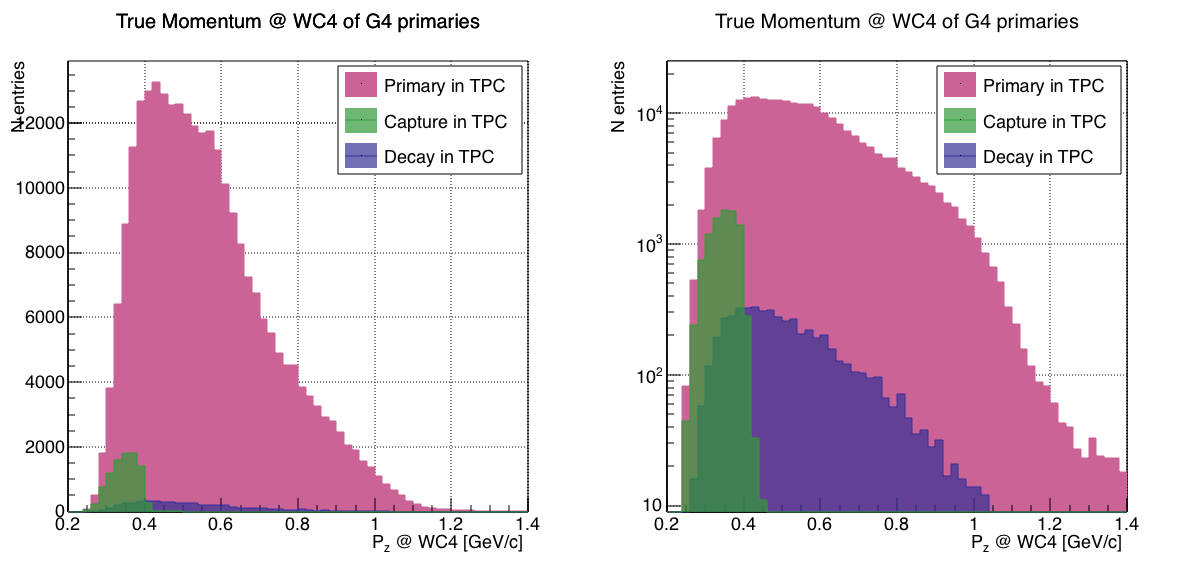
\includegraphics[width=15cm]{Chapter-7/Images/CDAsMomentumFunct.png}
\caption{True momentum distribution at wire chamber 4 for every simulated pion arriving in the TPC (pink), ending its life in capture (green) or in decay (blue) in the TPC, linear vertical axis on the left, logarithmic on the right. }
\label{fig:CaptureMom}
\end{figure}


In order to choose the selection value for the wire chamber momentum, it is beneficial to estimate the ratio of events which capture or decay that survive the selection in MC as a function of the momentum threshold, and compare it with the survival ratio for all events. This is done in figure \ref{fig:survRatio}. We define the survival ratio simply  as the number of events surviving the true momentum selection divided by the number of events of that category. We calculate the survival ratio separately for the three event categories explained above: total (pink), capture (green) and decay (blue).
Selecting pions with momentum greater than 420 MeV/c reduces the capture events by ~99\% while maintaining about 80\% of the total data sample. 
Figure \ref{fig:evtRatio} shows the ratio of events which end their life in capture (green) or decay (blue) over the total number of events as a as a function of the true momentum at wire chamber four. This ratio is slightly dependent on the inelastic cross section implemented in Geant4, as we are able to register a pion capture (or decay) only if it did not interact inelastically in the TPC. We choose a momentum threshold of 420~MeV/c because the percentage of capture events drops below 1\% and the percentage of decays is never above 2\% for momenta greater than 420~MeV/c.

\begin{figure}[h!]
\centering
\begin{minipage}[t]{0.45\textwidth}
\centering
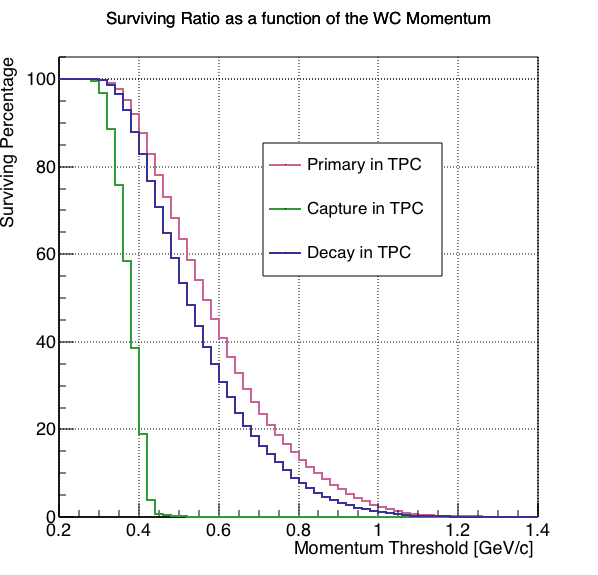
\includegraphics[width=7.5cm]{Chapter-7/Images/CDThreshold.png}
\caption{Survival ratio as a function of selection threshold on true momentum at wire chamber four for for every simulated pion arriving in the TPC (pink), capture (green) or in decay (blue).   }
\label{fig:survRatio}
\end{minipage}\hfill
\begin{minipage}[t]{0.45\textwidth}
\centering
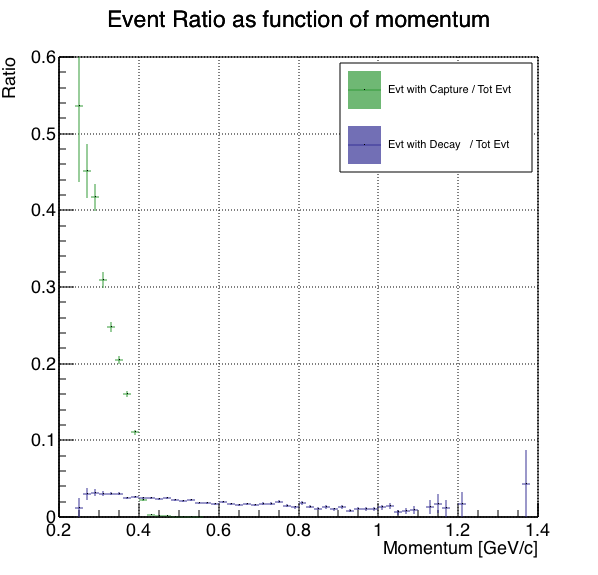
\includegraphics[width=7.5cm]{Chapter-7/Images/CDRatio.png}
\caption{Ratio between the capture (green) and decay (blue) events over the total number of events as a as a function of the true momentum at wire chamber four.}
\label{fig:evtRatio}
\end{minipage}
\end{figure}


